\section{Random Matrix filtering}
\label{sec:rmt}

\subsection{Empirical eigenspectrum}

The RMT analysis is the bridge between raw correlations and filtered networks. It asks how many collective modes are distinguishable from random-matrix noise. The core historical matrix uses $N=58$ assets and $T=1527$ observations, giving $Q=T/N\approx26.33$. The Marcenko--Pastur bounds are $\lambda_-=0.6482$ and $\lambda_+=1.4278$.

\begin{table}
\centering
\caption{RMT summary for the core historical universe.}
\label{tab:rmt_summary}
\resizebox{\linewidth}{!}{%
\begin{tabular}{rrrrrrrrrrrr}
\toprule
$N$ & $T$ & $Q$ & $\lambda_-$ & $\lambda_+$ & $\lambda_1$ & $\lambda_2$ & $\lambda_3$ & $\lambda_4$ & $\lambda_5$ & Above $\lambda_+$ \\
\midrule
58 & 1527 & 26.33 & 0.6482 & 1.4278 & 21.6505 & 3.0957 & 1.7839 & 1.6543 & 1.4835 & 5 \\
\bottomrule
\end{tabular}}
\end{table}
\FloatBarrier

Figure~\ref{fig:rmt_spectrum} shows the empirical spectrum against the random benchmark. The largest eigenvalue is far outside the Marcenko--Pastur band. Four additional eigenvalues also lie above the upper edge, suggesting that the correlation matrix contains a dominant market mode plus a small number of group or sector modes.

\begin{figure}
\centering

\includegraphics[width=0.88\linewidth]{images/figure_6_rmt_eigenvalue_spectrum.pdf}
\caption{Empirical eigenvalue spectrum and Marcenko--Pastur bounds. The largest eigenvalue is far outside the random band and is interpreted as the Market Mode.}
\label{fig:rmt_spectrum}
\end{figure}
\FloatBarrier

\subsection{Market Mode and significant eigenvalues}

The largest eigenvalue is 21.6505, corresponding to approximately 37.3\% of the total trace of the correlation matrix. This is the Market Mode. It captures broad co-movement and explains why the original correlation matrix has a strong positive common component. The next four eigenvalues are 3.0957, 1.7839, 1.6543 and 1.4835. These values are above $\lambda_+$ and are interpreted as candidates for group or sector structure.

The key methodological point is that the market mode is informative but also visually dominant. If a network is built directly from the original matrix, many edges can reflect market-wide co-movement rather than local structure. The group-mode matrix is therefore constructed to ask what remains after the broad common component is removed.

\subsection{Top eigenvector loadings}

Eigenvalues identify the strength of collective modes, but eigenvectors help interpret their composition. Figure~\ref{fig:eigenvector_loadings} reports top loadings for the leading eigenvectors. The first eigenvector is interpreted as the Market Mode. Subsequent eigenvectors are interpreted cautiously as group modes associated with sectors or localized dependency channels.

\begin{figure}
\centering

\includegraphics[width=\linewidth]{images/figure_7b_rmt_top_eigenvectors_top_loadings.pdf}
\caption{Top eigenvector loadings for the leading RMT modes. Eigenvector 1 corresponds to the Market Mode; subsequent eigenvectors are interpreted as group or localized sectoral components.}
\label{fig:eigenvector_loadings}
\end{figure}
\FloatBarrier

The second eigenvector is consistent with a Basic Materials and commodity-related component. The third contains financial and cross-sector structure. The fourth and fifth eigenvectors are more localized, with Telecommunications and Utilities-like components appearing among the dominant loadings. These labels are economic interpretations of the loading patterns. They should not be treated as mechanical classifications, because eigenvectors can mix sectors when firms share macroeconomic or liquidity exposures. The signs of eigenvector loadings are arbitrary up to multiplication by $-1$; therefore, interpretation focuses on relative grouping and magnitude rather than sign alone.

\subsection{Matrix reconstruction}

The spectral decomposition is numerically stable. Table~\ref{tab:rmt_reconstruction} reports reconstruction diagnostics. The Frobenius reconstruction error is approximately $2.74\times10^{-14}$, and the maximum absolute reconstruction error is approximately $3.99\times10^{-15}$. The diagonal of the filtered matrix is exactly 1.0 for all assets, confirming that the spectral reconstruction does not introduce numerical artefacts. This check ensures that the subsequent network differences are caused by mode selection rather than numerical instability.

\begin{table}
\centering
\caption{RMT reconstruction diagnostics.}
\label{tab:rmt_reconstruction}
\begin{tabular}{lr}
\toprule
Diagnostic & Value \\
\midrule
Frobenius reconstruction error & $2.74\times10^{-14}$ \\
Maximum absolute reconstruction error & $3.99\times10^{-15}$ \\
$C_{\mathrm{filtered}}$ diagonal min & 1.0000 \\
$C_{\mathrm{filtered}}$ diagonal max & 1.0000 \\
Eigenvalues above $\lambda_+$ & 5 \\
Market-mode trace share & 0.3733 \\
\bottomrule
\end{tabular}
\end{table}
\FloatBarrier

Figure~\ref{fig:rmt_filtered_matrices} shows the resulting matrix components. The original matrix combines all modes. The market-mode matrix captures broad positive co-movement. The group-mode matrix highlights weaker localized blocks after the market mode is removed. The noise component contains the random-band contribution, and the filtered matrix recombines the informative modes.

\begin{figure}
\centering
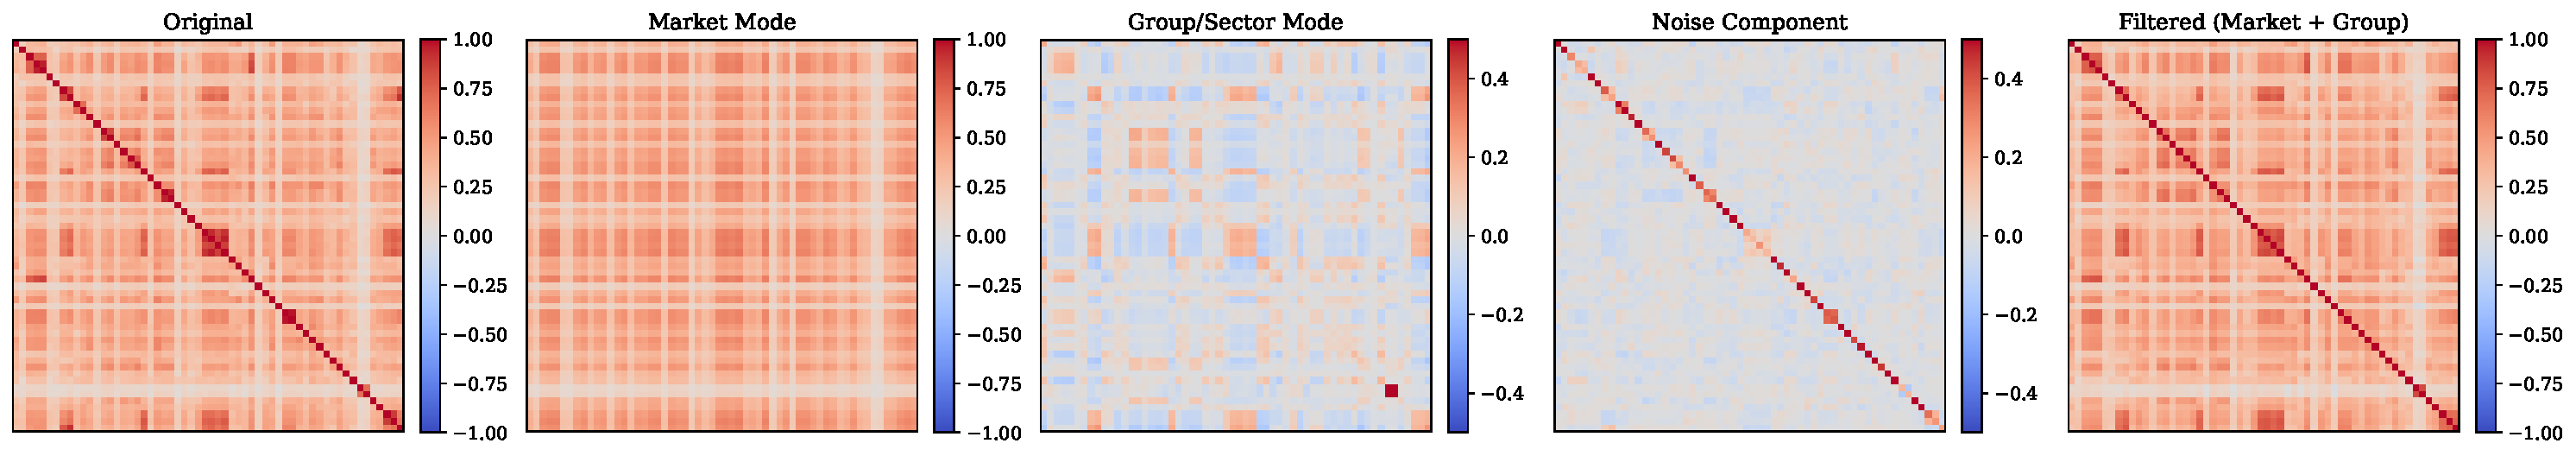
\includegraphics[width=\linewidth]{images/figure_8_rmt_filtered_matrices.pdf}
\caption{RMT-filtered matrix components. The decomposition separates original correlations into market, group/sector, noise and filtered components.}
\label{fig:rmt_filtered_matrices}
\end{figure}
\FloatBarrier

The important empirical result is not only that the market mode is large. It is that the group-mode matrix remains structured after removing it. This residual structure motivates the clustering and network sections: if localized dependency blocks remain, MST and PMFG topologies should change when built from the group-mode matrix.
